%\setchapterimage[6cm]{images/cabecera2}
%\setchapterpreamble[u]{\margintoc}
%%%%%%%%%%%%%%%%%%%%%%%%%%%%%%%%%%%%%%%%%%%%%%%%%%%%%%%%%%%%%

\chapter{Tiempo y Consenso Distribuido}
\label{ch:Tiempo y Consenso Distribuido}
\index{Tiempo y Consenso Distribuido}

 
 \section{Tiempo}
 \index{tiempo} \index{sincronización}
 
 
   Un sistema distribuido consta \cite{Coulouris2011} de en una colección   de $N$ procesos que puede expresarse como:  $N \quad procesos,  \quad p_{i} \quad  i = 1, 2,3,... N\quad  $.
 Cada proceso se ejecuta en un único procesador, y los procesadores no comparten memoria. 
 A su vez, cada proceso $p_{i} \quad en \quad P$  tiene un estado que se transforma a medida que ejecuta.  Incluye los valores de toda las variables internas y cualquier objeto en el entorno de sistema operativo local que afecta, como los archivos. 
 A medida que se ejecuta cada proceso  $p_{i}$ , toma acciones, las cuales son operación de envío o recepción de mensajes, u operaciones que transforma el estado de $p_{i}$
 
 Por ejemplo, si los procesos participan en una aplicación de comercio electrónico, entonces las acciones  pueden ser \textit{Mensaje de pedido enviado por el cliente} o \textit{transacción en el servidor del comerciante para iniciar sesión}.	
 
 Un \gls{evento} es la ocurrencia de una sola acción que conlleva un proceso \textit{fuera de su ejecuci\'on}  a medida que se ejecuta: una acción de comunicación o una acción que transforma el estado del sistema como todo.
 La secuencia de eventos dentro de un solo proceso,  se puede colocar en un único pedido total, que se denota por la relación  $ i $ entre los eventos. Es decir, $e-->_{i}e'$  si  y  solo  si  el  evento  $e$  	ocurre antes de $e’ \ en \ p_{i}$. 
 
Al la serie de eventos $e_{i}$  que se colocan dentro de un procesos $p_{i}$ se le llama \gls{historia del proceso} \cite{Coulouris2011} , ordenado  por la relación ${i}:$ \\  $history(p_{i})  = h_{i}  = <e_{i}^{0},  <e_{i}^{1},  <e_{i}^{2}, ....>  $ .

 
%  La sincronización de relojes en un sistema distribuido se utiliza para forzar un orden parcial o total en la ejecución de procesos y eventos del sistema. 
    
 La sincronización de relojes 	\cite{Czaja2018} \cite{Raptis2020} \cite{Vitillo2021}  en un sistema distribuido consiste en garantizar que los procesos  $p_{i}$ se ejecuten de forma cronológica y a la misma vez respetar el orden de los eventos $e_{i}$ dentro del sistema, es decir la historia del proceso.  La sincronización del reloj  $c_{i}$ es un método para sincronizar los valores del reloj de los nodos en un sistema distribuido con el uso de un reloj de referencia externo o un valor de reloj interno. 
	 
	
	 
	 \begin{tcolorbox}
	 	[colback=green!5!white,colframe=green!75!black,fonttitle=\bfseries, title=Tipos de sincronización de relojes físicos]
	 	Existen dos tipos de sincronización de relojes físicos:
	 	
	 	\begin{description}
	 		\item  [Sincronización externa]. Consiste en sincronizar los relojes  $c_{i}$ de los procesos  $p_{i}$ con una fuente de tiempo externa fiable, $S(t)$ para un  límite de sincronización $D$, de manera que:
	 		
	 		$	|S(t) – C_{i}(t)| < D $ ; siendo $D$ un límite mayor que cero y $S$ una fuente de tiempo UTC.
	 		
	 		\item  [Sincronización interna]: Si los relojes  $c_{i}$ están sincronizados entre ellos con un conocido grado de precisión y no necesariamente sincronizados con una fuente externa de tiempo:
	 		
	 		$|C_{i}(t) -C_{j}(t) | < D $ ; siendo $D$ un límite mayor que cero.
	 	\end{description}
	 	 
	 \end{tcolorbox}
	 
	 
	 El envió de mensajes entre los sistemas distribuidos es una parte fundamental para su funcionamiento. La sincronización de relojes ya sean físicos o lógicos aseguran que los procesos se realicen de manera secuencial y ordenada. 
	
\subsection{Relojes F\'isicos }	
 
	\index{reloj} 	\index{reloj f\'isico}
	
	  Los \gls{relojes} son dispositivos electrónicos que cuentan las oscilaciones que ocurren en un cristal a con una frecuencia definida, y generalmente dividen este recuento y almacenana el resultado en un contador de registro. 
	 Los dispositivos de reloj se pueden programar para generar interrupciones a intervalos regulares  para que, por ejemplo, implementar la división de tiempo.
	  En las computadoras   el sistema operativo lee el valor del reloj de hardware del nodo, lo escala y agrega un desplazamiento para producir un reloj de software  que aproximadamente mide el tiempo físico real $t$ para el proceso $p_{i}$. 
	
	\subsubsection{Sesgo y deriva del Reloj}
		\index{sesgo del reloj}
		\index{deriva del reloj}
		  Los relojes de computadora, cualquiera, tienden a no estar en perfecto acuerdo. 
		 La diferencia instantánea entre las lecturas de dos relojes se llama su \textbf{sesgo}. 
		 Los relojes a base de cristal utilizados en las computadoras están, cualquiera, sujetos a la \gls{deriva de reloj}, lo que significa que cuentan el tiempo a diferentes velocidades muy divergente. esto es debido a los que un reloj no marcha exactamente a la misma velocidad que otro, lo que significa, que después de cierto tiempo la hora indicada por el reloj se irá separando  de la indicada por el otro reloj, ver Figura \ref{fig:sesgo-derv} que ilustra las diferncias de hora que se podr\'ian generar en consecuencia.
	
	
	\begin{figure}%
			\begin{center}
		\includegraphics[width=0.8\linewidth] {8/9.png} 
		\caption{Sesgo y deriva del reloj}
		\label{fig:sesgo-derv}
			\end{center}
	\end{figure}
	
	 
	\subsubsection{UTC}
 	\index{UTC}
 
			 La hora universal coordinada,  \textbf{UTC}   es un estándar internacional para el cronometraje.  Las señales UTC se sincronizan y transmiten regularmente desde estaciones terrenas de radio y satélites que cubren muchas partes del mundo. 
			 Las fuentes satelitales incluyen el Sistema de Posicionamiento Global (\textbf{GPS, Global Positioning System}). Dependiendo de la estación utilizada. Las señales recibidas de los satélites GPS tienen una precisión de aproximadamente 1 microsegundo. 
			  Las computadoras con receptores conectados pueden sincronizar sus relojes con estas señales de tiempo.
		 
		
		
		\subsubsection{Algoritmo de Cristian}
			\index{reloj f\'isico}
				\index{algoritmo de Cristian}
			

			%-------------------------------------------------------------------
			Un ejemplo de sincronizai\'on externa es el algoritmo de sincronizaci\'on de relojes de Cristian.
			
		El Algoritmo de Cristian \cite{Cristian1989}  propone sincronizar un conjunto de relojes de 	máquinas a partir de una que esté sincronizada externamente (tiempo u hora real), a través de la red de comunicaciones de datos entre computadoras. 
	
	 Se parte de un sistema distribuido con varios nodos $i$, cada uno de ellos cuenta con un reloj local $C_{i}$. En cualquier instante $t$ se cumple para todos los nodos $C_{i}(t) = t$, es decir, todos los relojes locales coinciden con  la misma hora.   Periódicamente cada máquina envía un mensaje para solicitar el tiempo actual a este servidor:
		
		\begin{itemize} 
		 			
		\item Un proceso $p$ hace una petición de tiempo al servidor en un mensaje $m_{r}$.
		\item El servidor responde con un mensaje $m_{t}$ en el que incluye su tiempo $t_{UTC}$.
		\item El proceso que recibe el mensaje  $m_{t}$  actualiza su reloj con el tiempo $t_{UTC}$,   
		
		\item Hay que considerar el error o demora ya que se ha requerido un tiempo para la transmisión del mensaje desde el servidor: se mide el tiempo que se tarda en recibir la respuesta desde que de envía el mensaje de petición, $t_{trans}$.
		 
		 \item \textit{El tiempo estimado de propagación será  $t_{trans}/2$  
		\item  El  cliente sincroniza su reloj a $t_{UTC} + t_{trans}/2$}	 
				 
		\end{itemize}
		
		 

\paragraph{Problemas con el Algoritmo de Cristian} 
			\begin{enumerate}
				\item  Si tiempo del emisor es mayor al valor de $t + T_{trans}$ 	 perjudicaría a los archivos compilados.
				\item  El tiempo de propagación $T_{trans}$, varía según la carga en la red.
				\item     Posibilidad de fallo debido a la existencia de un único servidor. Cristian sugiere múltiples servidores de tiempo sincronizados que suministren el tiempo. El cliente envía un mensaje de petición a todos los servidores y toma la primera respuesta recibida.
			\end{enumerate}
		
			En la Figura \ref{fig:Cristian} muestra el proceso del algorito y en la Figura \ref{fig:Cristian-tiempo} hay un esquema con el manejo  del tiempo entre el cliente y el servidor para sincronizarse usando el algoritmo de Cristian.	 
				
		 \begin{figure}%
		 		\begin{center}
		 	\includegraphics[width=0.8\linewidth] {8/7.png} 
		 	\caption{Algoritmo de Cristian}
		 	\label{fig:Cristian}
		 		\end{center}
		 \end{figure}
		  
			 
			Si se conoce el tiempo que tarda el servidor en manejar la interrupción ${t_{1}}$, la estimación de tiempo puede mejorar con base en la siguiente ex­presión: $ \dfrac{T_{1} - T_{0} - t_{1}}{2}$, que representa la  estimación del tiempo de propagación  realizado por el reloj de la máquina emisora.
			
			Cristian sugiere hacer varias mediciones para mejorar la precisión y descartar los valores límites de ${T_{1} - T_{0}}$, ya que estos están en función de la operación de la red.			 
					
			 \begin{figure}[h]%
			 		\begin{center}
				\includegraphics[width=0.8\linewidth] {8/8.png} 
				\caption{Tiempo en el Algoritmo de Cristian}
				\label{fig:Cristian-tiempo}
					\end{center}
			\end{figure}
			
				El algoritmo de Cristian es probabilístico ya que no garantiza que un procesador pueda 	leer un reloj remoto con una precisión específica. Indica que, intentando una cantidad de veces suficiente, la hora recuperada puede ser leída con una precisión dada, con una probabilidad cerca de uno, según lo deseado.
		
			%--------------------------------------------------------------------
			%--------------------------------------------------------------------
			
			\subsubsection{Algoritmo de Bekerley}
			\index{algoritmo de Bekerley}
			
			%--------------------------------------------------------------------
		 Algoritmo de Bekerley \cite{Gusella1985} es un algoritmo centralizado o de sincronizaci\'on interna, en el que  se elige un servidor  entre todos los equipos que se encuentran conectados en el entorno. Este servidor toma el rol de maestro o  servidor de tiempo y los servidores conectados son esclavos.  
		 
			El algoritmo de Bekerley,   opera de la siguiente manera: 
		 
	  \begin{itemize} 
			 
		\item 	El servidor de tiempo le envia a cada máquina su tiempo
		\item	Las máquinas cliente le indican el número de segundos que están adelantadas o retrasadas con respecto al tiempo del servidor, si es un número positivo entonces están adelantadas y si es negativo están atrasadas.
		\item	El servidor suma todos estos datos y los divide entre el número de máquinas incluyéndose él mismo.
		\item 	El resultado lo suma a su propio tiempo obteniendo $t$, y calcula el número de segundos que le falta o le sobra a una máquina para llegar a ese tiempo $t$, y se lo envía a la máquina. Lo mismo hace para cada máquina.
		\item	Las máquinas esclavas reciben el resultado y sincronizan su tiempo.	Cada equipo se limitará a actualizar su reloj adelantándolo en caso de ir con retraso o atrasándolo en caso de ir adelantado para aplicar la deriva recibida.				 
		\end{itemize}		
				
			%-----------------------------------------------------
			
			En la Figura \ref{fig:Bekerley} se ilustra como opera el algoritmo de Bekerley.
			
		\begin{figure}%
				\begin{center}
			\includegraphics [width=0.8\linewidth]{8/1.png} 
			\caption{ Algoritmo de Bekerley}
			\label{fig:Bekerley}
				\end{center}
		\end{figure}
		 
			%-------------------------------------------------------------------
			
			
		\subsubsection{Protocolo NTP}
			\index{protocolo NTP}
			
		Los algoritmos de 	Cristian y Berkeley son adecuados para redes rápidas y por lo tanto son usados principalmente para intranets.
		En \cite{Mills1995} Mills define un protocolo llamado NTP (NTP, Network Time Protocol) que es una una arquitectura y protocolo para distribuir «relojes»  
		NTP permitir la sincronización de los relojes de clientes en todo internet usando UTC. La latencia/retardo es significativa y variable
		
		Define una jerarquía dependiendo de la calidad del reloj
		
	En la Figura \ref{fig:NTP} se muestra un esquema de los niveles que establece el procolo basado en la calidad del Reloj. NTP usa los estratos 1 a 16 para definir la precisión del reloj. Un valor de estrato más bajo representa una mayor precisión. Los relojes en los estratos 1 a 15 están en estado sincronizado y los relojes en el estrato 16 no están sincronizados.
	Un servidor NTP de estrato 1 obtiene su hora de una fuente de tiempo autorizada, como un reloj atómico. Proporciona tiempo para otros dispositivos como servidor NTP principal. Un servidor de hora de estrato 2 recibe su hora de un servidor de hora de estrato 1, y así sucesivamente.
		
			\begin{figure}[h]%
					\begin{center}
					\includegraphics [width=0.8\linewidth] {8/3.png} 
					\caption{ Protocolo NTP. Adaptado de \href{http://www.h3c.com}{h3c} }
					\label{fig:NTP}
				\end{center}
		\end{figure}
		
	
		
	La sincronización entre cada par de elementos de la 	jerarquía se realiza mediante el siguiente proceso:
	\begin{itemize}
		\item  Modo multicast: Para redes LAN. Se transmite por la red a todos los elementos de forma periódica. Tiene una   precisión baja.
		\item Modo de llamada a procedimiento: Similar al algoritmo de Cristian. Se promedia el retardo de transmisión. Proporciona una mejor 	precisión.
		\item Modo simétrico: Los dos elementos intercambian mensajes de sincronización que ajustan los relojes. Tiene una mayor precisión.
	\end{itemize}
		 
		Para el intercambio de mensajes   entre los servidores se usa datagramas UDP.
			
		 
			%------------------------------------------------------------------
			\subsection{Relojes L\'ogicos}
						\index{reloj l\'ogico}
						
			A diferencia de los relojes f\'isicos que miden el tiempo real, los relojes l\'ogicos dan un marco de referencia de los eventos y del orden en el que ocurren.			
			La idea de un reloj lógico consiste en crear un sistema de convergencia del tiempo mediante la medición de las derivas, de manera que la noción de tiempo universal se sustituye por la noción de un tiempoo global auto-ajustable. Los relojes lógicos son útiles para ordenar eventos en ausencia de un reloj común.
			
			A continuaci\'on se detallan dos algoritmos basado en relojes l\'ogicos: algoritmo de Lamport y algoritmo de los relojes vectoriales.
		 
			\subsubsection{Algoritmo de Lamport}	
						\index{algoritmo de relojes l\'ogicos de Lamport}
			%--------------------------------------------------------------------
			 
				 
			Lamport,  \cite{Raptis2020} \cite{Czaja2018} \cite{Lamport1978},  señala que la sincronización de relojes no tiene que ser absoluta. Si dos procesos no interactúan no es necesario que sus relojes estén sincronizados. 
			Indica que es importante que  los procesos coincidan en el orden en el cual ocurren los eventos. No interesa  que los procesos  concuerden de manera exacta en la hora.
			En ciertos  algoritmos lo que  importa es la consistencia interna de los relojes, no su particular cercanía al tiempo.
				 
			%--------------------------------------------------------------------
			%--------------------------------------------------------------------
			
			El Algoritmo de los relojes l\'ogicos de Lamport  define una relación llamada \textit{\textbf{a ocurre antes de b}}  representada por  $a \rightarrow b$. Esta relación se puede observar de manera directa en dos situaciones:
				
						
						 \begin{tcolorbox}
							[colback=red!5!white,colframe=red!75!black,fonttitle=\bfseries, title=Algoritmo de los relojes l\'ogicos de Lamport]
							\begin{enumerate}
								\item Si $a,  b$  son eventos en el mismo proceso y $ a$ \textbf{\textit{ocurre antes de}} $b$, entonces  $ a \rightarrow b $ es verdadero.
								\item Si $a$ es el evento de envío de un mensaje por un proceso y $b$ es el evento de la recepción del mensaje por otro proceso, entonces  $ a \rightarrow b $ también es verdadero. Un mensaje no puede recibirse antes de ser enviado, o incluso al mismo tiempo en que es enviado, ya 	que necesita cierta cantidad de tiempo finita, diferente de cero, para llegar.
							\end{enumerate} 
						\end{tcolorbox}
						
					 
			  La ocurrencia anterior es una relación transitiva, por lo que si   $ a \rightarrow b $  y   $ b \rightarrow c $ , entonces  $ a \rightarrow c $ .
				  Si dos eventos, $x,  y$, ocurren en diferentes procesos que \textbf{no} intercambian mensajes, entonces  $ x \rightarrow y $  no es verdadera, pero tampoco  $ y \rightarrow x $ .
			Se dice que estos eventos son  \gls{eventos concurrentes}.
			
				\begin{figure}%
						\begin{center}
				\includegraphics[width=0.8\linewidth]{8/4.png} 
				\caption{Eventos concurrentes}
				\label{fig:Lamport-conc}
					\end{center}
			\end{figure}
			
			Por ejemplo, en la Figura \ref{fig:Lamport-conc} los eventos $a$, $b$ y $c$ son eventos con relaciones transitivas al igua que los eventos  $a$, $b$ y $f$. Por otra parte entre los eventos  $a$ y $e$ no se puede establecer alg\'un tipo de relaci\'on por tanto son eventos concurrentes
			 	
			%--------------------------------------------------------------------
			%--------------------------------------------------------------------
			\paragraph{Implementaci\'on de relojes lógicos de Lamport}
			
		Para implementar los relojes lógicos de Lamport, cada proceso $P_{i}$ mantiene un contador local $C_{i}$
					
		\begin{enumerate} 
			\item  Antes de ejecutar un evento , $P_{i}$  ejecuta $C_{i}$ $\leftarrow$ $ C_{i} + 1 $
			\item Cuando el proceso $P_{i}$ envía un mensaje $m$ a $P_{j}$, éste ajusta el registro de tiempo de $ m, ts(m)$ , igual a $C_{i}$ después de haber ejecutado el paso anterior.
			\item Al recibir mensaje $ m $, el proceso $P_{j}$ ajusta su  contador local a $C_{j}$ $\leftarrow $  $max{C_{j}, ts(m)}+1$, después de lo cual ejecuta el primer paso y entrega el mensaje a la aplicación.
		\end{enumerate}		
			
			
		Un ejemplo de  la  implementaci\'on del algoritmo de Lamport se muestra en la Figura \ref{fig:Lamport-ejem1}. Cuando un proceso $p$ genera un evento, $C_{i}$ $\leftarrow$ $ C_{i} + 1 $  
		 Cuando un proceso envía un mensaje incluye el valor de su reloj
		Y cuando un proceso $q$ recibe un mensaje $m$con un valor $t$, $q$ ajusta su relos en  $C_{j}$ $\leftarrow $  $max{C_{j}, ts(m)}+1$
	 
			
		\begin{figure}%
				\begin{center}
			\includegraphics[width=0.8\linewidth] {8/6.png} 
			\caption{Ejemplo del  Algoritmo de Lamport. }
			\label{fig:Lamport-ejem1}
				\end{center}
		\end{figure}
		
	\paragraph{Sincronizaci\'on en Algoritmo de Lamport}		
		La sincronizaci\'on en el algoritmo de lo relojes l\'ogico de Lamport entre procesos puede visualizarse en el ejemplo de la Figura \ref{fig:Lamport-sincro}, parte a:
			
		\begin{itemize} 
		
			\item En el tiempo 6, el proceso $P1$ envía  mensaje $m1$ al proceso $P2$.  El reloj del proceso $P2$ ajusta a  16 al llegar el mensaje. 
			\item Mensaje $m2$ desde $P2$ hasta $P3$ se lleva 16 marcas de tiempo
			\item Mensaje $m3$ deja  proceso $P3$ en 60 y llega a $P2$ en 56. Y  mensaje $m4$ hasta $P1$ llega en 54. 
		\end{itemize}
		Estos valores son imposibles. Indica que esos procesos no est\'an sincronizados.
		En la parte b de la  Figura \ref{fig:Lamport-sincro} se muestra como deber\'ia ser la marca de tiempo en procesos sincronizados.
		
			\begin{figure}%
					\begin{center}
			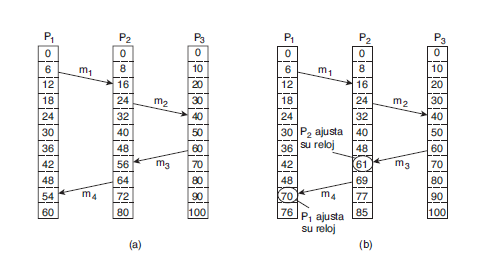
\includegraphics[width=0.8\linewidth] {8/lamport-11} 
			\caption{Sincronizaci\'on en el  Algoritmo de Lamport. Tomado de \cite{Steen2017} }
			\label{fig:Lamport-sincro}
				\end{center}
		\end{figure}
		
		
	\paragraph{Problemas con el algoritmo de Lamport}
	
			\begin{itemize}	
				\item Con los relojes de Lamport, nada puede decirse sobre la relación entre dos eventos $a$ y $ b$ si se compara los valores de tiempo $C(a)$ y  $ C(b)$.  En otras  palabras, si $C(a) le C(b) $, entonces esto no necesariamente implica que $a$ realmente ocurrió antes que $b$.
				
				\item Relojes lógicos de Lamport   representan una relación de orden parcial. El orden parcial en la Figura \ref{fig:Lamport-ejem1} es {a, e, i }, {b, j }, {f, k }, {c, g }, {h, l }, {d, m}
						
			\end{itemize}
			  %-------------------------------------------------------------------------------------
			
			%------------------------------------------------------------------
			\subsubsection{Algoritmo  de Relojes Vectoriales}	
			 
				\index{algoritmo  de relojes vectoriales}
			%--------------------------------------------------------------------
		 En distintos documentos, \cite{Mattern1989} y \cite{Fidge1991} proponen  una solución para superar las dificultades que presenta el Algoritmo de relojes l\'ogicos de Lamport. 

		\begin{itemize} 
			\item  Un reloj vectorial, $VC(a)$, asignado a un evento $a$, tiene la propiedad de que si $ VC(a) < VC(b) $ para algún evento $ b$, entonces se sabe que el evento $a$ precede en causalidad al evento $b$
			\item  Los relojes vectoriales se construyen de manera que cada proceso  $P_{i}$ mantenga un vector $VC_{i}$ con las dos siguientes propiedades:
			
				\begin{enumerate}
					\item  $VCi[i]$ es el número de eventos que han ocurrido hasta el momento en $P_{i}$. En otras palabras, $	VCi[i] $ es el \textbf{reloj lógico} del proceso $P_{i}$.
					\item  Si $VCi[j] =  k$ , entonces $P_{i}$ sabe que han ocurrido $ k$ eventos en $P_{j}$. Así, éste es el conocimiento
					de $P_{i}$ del tiempo local en $P_{j}$.
				\end{enumerate}
		\end{itemize}		
				
		\paragraph{Implementaci\'on de 	Relojes Vectoriales}		
			 
		Se realizan los siguientes pasos:
					
	\begin{enumerate} 
		\item  Antes de ejecutar un evento,  $P_{i}$  ejecuta $VC_{i}[i] \leftarrow VC_{i}[i] + 1 $ .
		\item Cuando el proceso $P_{i}$ envía un mensaje $m$ a $P_{j}$, éste establece el registro de tiempo de
		$m, ts(m)$, igual a $VC_{i}$ después de haber ejecutado el paso anterior.
		\item Una vez que se recibe el mensaje $m$, el proceso $P_{j}$ ajusta su propio vector configurando
		$VC_{j}[k] \leftarrow max{VC_{j}[k],ts(m)[k]} $ para cada $k$ , después de lo cual ejecuta el primer 	paso y libera el mensaje a la aplicación.
	\end{enumerate}		
			 
			%--------------------------------------------------------------------
	\paragraph{Relojes Vectoriales. Ejemplo} 
	
	Por medio de este mecanismo de Relpjes Vectoriales  siempre es posible evaluar 	si dos marcas de tiempo tienen o no relación de precedencia.
	Basado en la Figura \ref{fig:Vectorial-1} se puede decir que:
	
	\begin{itemize}
	\itemsep=2pt\topsep=2pt\partopsep=2pt
	\parskip=2pt\parsep=2pt
	\item $a$  $\rightarrow b \: \Leftrightarrow \: V_{a} <  V_{b}$
	\item $V_{a} <  V_{b}    \:     \Leftrightarrow \:  V_{a}  \leq  V_{b}   \wedge \:   V_{a} \neq  V_{b} $
	
	\item $V_{a} \leq  V_{b}   \: \Leftrightarrow \:	 V_{a}[i]   \leq  V_{b}[i]  ,\: \forall \: i \: \in ^{} [1, \dotsb , N] $

 	\item $V_{a} = V_{b}  \: \Leftrightarrow \:  V_{a}[i]  =  V_{b}[i] , \:  \forall \: i \: \in [1,\dotsb, N] $
 
	\end{itemize}
			
			
	Por tanto mediante los vectores de relojes se puede
	establecer la precedencia o concurrencia de dos eventos
	
	\begin{itemize}
		\itemsep=2pt\topsep=2pt\partopsep=2pt
		\parskip=2pt\parsep=2pt
		
		\item $ V_{a} \leq  V_{b} $ \: $\Leftrightarrow$ \: ${a} \rightarrow {b}$  
	
		\item $ V_{b} \leq  V_{a} $ \: $\Leftrightarrow$ \: ${b}  \rightarrow {a}$  
		
		\item $ {\overline{(V_{a} \le  V_{b})} }$  $\land$ $\overline{(V_{b} \le  V_{a})}$  \: $\Leftrightarrow$ \: $ a \shortparallel b$

	\end{itemize}
	
	Por ejemplo, en la Figura \ref{fig:Vectorial-1} ?` qu\'e se podr\'ia decir acerca de los procesos $a$ y $m$ ?
	
		
	\begin{figure}[h]%
			\begin{center}
		\includegraphics[width=0.8\linewidth] {8/5.png} 
		\caption{Ejemplo del  Algoritmo  Vectorial.}
		\label{fig:Vectorial-1}
			\end{center}
	\end{figure}

El proceso $a \rightarrow (1,0,0) $  y el proceso $m \rightarrow (2,3,5)$ de all\'i: $1 \leq 2 $ \:$\land$\:  $0 \leq 3 $  \:$\land$\:  $0 \leq 5 $ \:  $\land$  \: NOT ($1 = 2 $ \:$\land$\:  $0 = 3 $  \: $\land$\:  $0 = 5 $). Por lo tanto $a$ ocurre antes que $m. \:  a \rightarrow m$

?` Y con respecto a los procesos  $c$ y $m$ ?


El proceso $c \rightarrow (3,0,3) $  y el proceso $m \rightarrow (2,3,5)$,  de all\'i: $3 \leq 2 $ \:$\land$\:  $0 \leq 3 $  \:$\land$\:  $3 \leq 5 $ \:  $\land$  \: NOT ($3 = 2 $ \:$\land$\:  $0 = 3 $  \: $\land$\:  $3 = 5 $) no se cumple, entonces  es falso que $ V_{c} \leq  V_{m} $. 


De la misma manera, con respecto a los procesos $m $ y $c$:
 
 $2 \leq 3 $ \:$\land$\:  $3 \leq 0 $  \:$\land$\:  $5 \leq 3 $ \:  $\land$  \: NOT ($2 = 3 $ \:$\land$\:  $3 = 0 $  \: $\land$\:  $5 = 3 $) no se cumple,  entonces es falso que  $ V_{m} \leq  V_{c} $.
Por lo tanto $c$ es concurrente con $m. \: a\shortparallel m$.  
  
				
				
	\paragraph{Uso de los Relojes Lógicos}
	Los  relojes lógicos de Lamport o los  Vectoriales, se  aplican a:
    \begin{itemize}
    	\item 	Mensajes periódicos de sincronización.
		\item Campo adicional en los mensajes intercambiados
	 \end{itemize}
	Por medio de relojes lógicos se pueden resolver el orden de los  eventos  considerando factores como  prioridad o
	equitatividad.	Tambi\'en, se puede detectar violaciones de causalidad.
%%%%%%%%%%%%%%%%%%%%%%%%%%%%%%%%%%%%%%%%%%%%%%%%%%%%%%%%%%%%%%%%%%%%%%%%%%%%%%%%%%%%%%%%%%%%%%%%%%%%%%%%%%%%%%%%%%%%%%%%%%%%%%%%%%%%
\section{Consenso Distribuido}
\index{consenso distribuido}


	En los sistemas distribuidos resultan fundamentales la concurrencia y la colaboración entre diversos 	procesos. La \gls{concurrencia} es la capacidad de ejecutar varios procesos simultáneamente, es decir, la existencia de más de un proceso en  períodos de tiempo superpuestos.
	
	Los procesos necesitan el acceso simultáneo a los mismos recursos. Para  evitar que tales accesos concurrentes corrompan los recursos, o los vuelvan inconsistentes, se necesita encontrar soluciones que garanticen que los	procesos tengan acceso mutuamente exclusivo.
   
   La exclusión mutua garantiza que los procesos concurrentes   puedan compartir recursos. A continuaci\'on  se presentanlos las soluciones  relacionados con el problema de la exclusión mutua \cite{Wu1998} \cite{Czaja2018}.
 
\subsection{Algoritmos basados en Token}
%--------------------------------------------------------------------
\index{ algoritmos basados en token}
\index{ exclusi\'on mutua}

Estos algoritmos logran la exclusión mutua pasando un mensaje especial entre los procesos llamado token \cite{Steen2017}. Solo hay un token disponible y solo aquel proceso que lo tenga podrá entrar en la región crítica.
 Las soluciones basadas en Token usan la siguiente estrategia para garantizar el acceso exclusivo a recursos compartidos:
	\begin{itemize} 
		\item La exclusión mutua se logra pasando entre los procesos un mensaje especial conocido como \textit{token}. 
		\item Sólo hay un \textit{token} disponible, y quien lo tenga puede acceder al recurso compartido.
		\item  Cuando termina, el \textit{token} pasa al siguiente proceso. 
		\item Si un proceso 	tiene el \textit{token} pero no está interesado en acceder al recurso, simplemente lo pasa el \textit{token} al siguiente proceso.
		
	\end{itemize}
 
 
 La \gls{inanicion} y el \gls{interbloqueo} son las situaciones que se deben  evitar cuando se usa  las soluciones basadas en \textit{token}:
	\begin{itemize} 
		\item De acuerdo con la organización de los procesos, éstos pueden garantizar fácilmente que todos tendrán la oportunidad de acceder a los recursos. En otras palabras, evitan la inanición.
		\item  Interbloqueo mediante los cuales diversos procesos se esperan unos a otros para continuar pueden evitarse fácilmente, 	contribuyendo a su simplicidad. 
		
	\end{itemize}
 
 La desventaja de las soluciones basadas en \textit{token} suceden  en el caso de cuando el \textit{token}  se pierde (por ejemplo, debido a que falla del proceso que lo tiene), entonces es necesario iniciar un intrincado proceso distribuido para garantizar la creación de un nuevo \textit{token}, pero sobre todo, para que sea el único \textit{token}.
 

 
%---------------------------------------------------------------------

\subsubsection{Algoritmo de Servidor Central}
%--------------------------------------------------------------------
%\index{algoritmos basados en token!algoritmo servidor central}
\index{ algoritmo servidor central}

Una solución simple para la exclusión mutua distribuida utiliza un coordinador \cite{Steen2017} \cite{Coulouris2011} \cite{Wu1998}. Para cada proceso que solicita el acceso a la
sección crítica, se envía su solicitud al coordinador que pone en cola todas las solicitudes y les otorga permiso en función de una determinada regla, por ejemplo, en función de sus marcas de tiempo. En la Figura \ref{fig:alg-serv-central} se ilustra el comportamiento de algoritmo del servidor central. 

 
\begin{figure}[h]%
		\begin{center}
	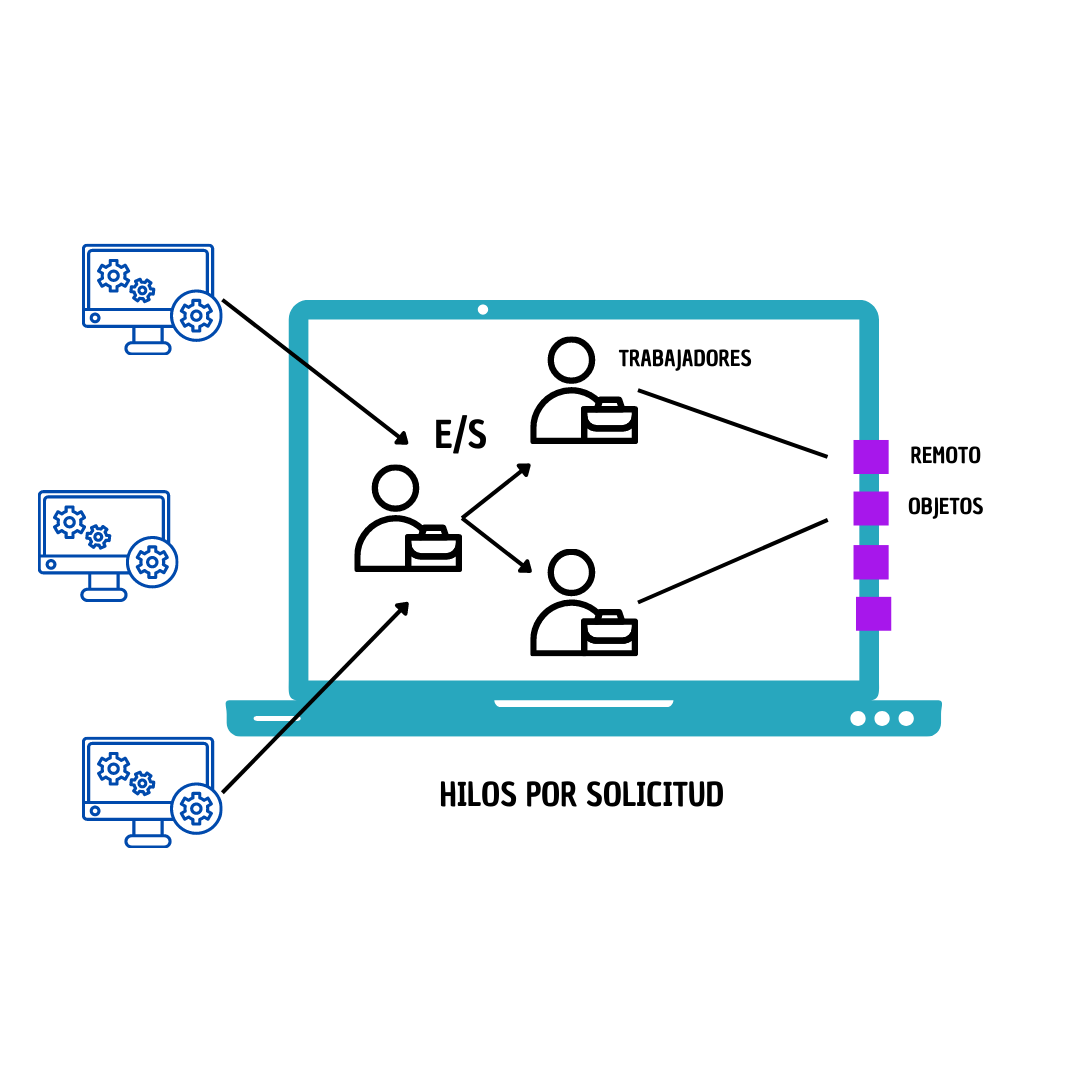
\includegraphics [width=0.8\linewidth]{8/C/2.png} 
	\caption{ Algoritmo de Servidor Central.}
	\label{fig:alg-serv-central}
		\end{center}
\end{figure}


Los problemas con este algoritmo se presentan cuando el coordinador falla o cuando falla el poseedor del token. Tambi\'en un solo coordinador en un gran sistema puede ocasionar un embotellamiento. 
%---------------------------------------------------------------------
\subsubsection{Algoritmo Anillo de Procesos}
%----------------------------------------------------------------------
 El algoritmo de Anillos de Procesos \cite{Coulouris2011} \cite{Steen2017}, Figura \ref{fig:alg-anillo} opera de la siguiente manera: 
	\begin{itemize} 
		\item Al arrancar el sistema, al proceso de posición $1$ se le da un token, el cual irá circulando por el anillo.
		\item Cuando el proceso $ k$ tenga el token, debe transferirlo mediante un mensaje al proceso $k+1$.  Así, el token irá pasando por todos los nodos del anillo.
		\item Cuando un proceso recibe el token, si quiere entrar a la región crítica, retiene el token y entra en la región crítica.
		\item Cuando el proceso sale de la región crítica le pasa el token al siguiente nodo del anillo
	\end{itemize}
 
	
	
\begin{figure}[h]%
		\begin{center}
	\includegraphics[width=0.8\linewidth] {8/C/1.png} 
	\caption{ Algoritmo de Anillo de Procesos.}
	\label{fig:alg-anillo}
		\end{center}
\end{figure}

Los inconvenienetes con este algoritmo es que si falla  cualquiera de los nodos provocará el fallo del sistema completo, ya que romperá el anillo circular con el que se conectan todos los nodos.
Otra falla es que al acceso a la secci\'on cr\'itica no se logra  en el orden en el que los nodos se añaden al anillo, ya que depende del lugar donde se encuentre el token.  
 
%----------------------------------------------------------------------
\subsection{Algoritmos basados en Marcas de Tiempo}
%----------------------------------------------------------------------
\index{ algoritmos basados en marcas de tiempo}
 
%----------------------------------------------------------------------
Los algoritmos basados en marcas de tiempo  utiliza marcas de tiempo \textit{timestamps} en lugar de números de secuencia para ordenar las solicitudes de acceso a  la sección crítica.
Este enforque sigue este procedimiento:
	\begin{itemize} 
		\item Un sitio se comunica con otros sitios para determinar qué sitios deben ejecutar la sección crítica. Esto requiere 	el intercambio de dos o más rondas
		sucesivas de mensajes. 
	 
		\item Cada vez que un sitio solicita una sección crítica, recibe una marca de tiempo. La marca de tiempo también se	usa para resolver cualquier conflicto entre las solicitudes de sección crítica.
		\item Todo algoritmo que sigue un enfoque no basado en tokens mantiene un reloj lógico. Los relojes lógicos se actualizan  según el esquema de Lamport.
	\end{itemize}
 
 
 
%----------------------------------------------------------------------
\subsubsection{Algoritmo de Lamport de Exclusi\'on Mutua Distribuida }
%----------------------------------------------------------------------
\index{ algoritmo de Lamport de exclusi\'on mutua}

\index{ algoritmo de Lamport de exclusi\'on mutua}
 
 Es un algoritmo basado en permisos propuesto por Lamport, \cite{Lamport1978} como una ilustración de su esquema de sincronización para sistemas distribuidos. Es un  mecanismo basado en relojes lógicos para el orden  total de las peticiones en el sistema.
 Los permisos basados en la marca de tiempo \textit{timestamps} se utiliza para ordenar las solicitudes de sección crítica y para resolver cualquier conflicto entre las solicitudes.
 
 Cada nodo  mantiene una cola de peticiones que contiene las
 peticiones ordenadas por marcas de tiempo, y
 también tiene un conjunto de peticiones de los nodos
 que necesita permiso para entrar en su región crítica.
 El algoritmo requiere que los mensajes se entreguen
 en orden FIFO entre cada par de nodos.   	
	
El acceso a la secci\'on cr\'itica se orden en orden creciente en marcas de tiempo, considerando el menor valor como prioritario.
Es decir, una solicitud con una marca de tiempo más pequeña tendrá permiso para ejecutar la sección crítica 	primero que una solicitud con una marca 	de tiempo más grande.
 
El algoritmo  opera as\'i:  
	\begin{itemize} 
		\item Se utilizan tres tipos de mensajes (SOLICITUD,
		RESPUESTA y LIBERACIÓN) y se supone que los
		canales de comunicación siguen el orden FIFO.
		\item Un sitio envía un mensaje de SOLICITUD a todos los
		demás sitios para obtener su permiso para ingresar a
		la sección crítica.
		\item Un sitio envía un mensaje de RESPUESTA al sitio que
		solicita el permiso para ingresar a la sección crítica.
		\item Un sitio envía un mensaje de LIBERACIÓN a todos los
		demás sitios al salir de la sección crítica.

		\item Cada sitio $S_{i}$ , mantiene una cola para almacenar
		solicitudes de secciones críticas ordenadas por sus
		marcas de tiempo Request($queue_{i}$) denota la cola del sitio 	$S_{i}$ .
		\item Se proporciona una marca de tiempo a cada solicitud de 	sección crítica utilizando el reloj lógico de Lamport. La marca de tiempo se utiliza para determinar la
		prioridad de las solicitudes de sección crítica. 
		\item La marca de tiempo más pequeña tiene mayor prioridad sobre la 	marca de tiempo más grande. La ejecución de la solicitud de sección crítica siempre está en el orden de su marca de tiempo.
	\end{itemize}
 
%----------------------------------------------------------------------
\paragraph{Acceso a la secci\'on cr\'itica}
	\begin{itemize} 
		\item  Si sitio $S_{j}$ desea ingresar a la sección
		crítica, envía un mensaje de solicitud  Request($t_{si},
		i$) a todos los demás sitios y coloca la solicitud en
		\textbf{Request}($queue_{i}$).   $t_{si} $ es la marca de
		tiempo de  $S_{ji}$ .
		\item Cuando  $S_{j}$  recibe el mensaje  	\textbf{REQUEST}($t_{si},i$) del sitio  $S_{i}$, devuelve un mensaje \textbf{REPLY} con marca de tiempo al sitio $S_{i}$ y coloca la solicitud del sitio  $S_{j}$ en \textbf{Request}($ queue_{j}$). 				   
	\end{itemize}
 
%----------------------------------------------------------------------
{\paragraph{Ejecutar en la secci\'on cr\'itica} 
	\begin{itemize}
		\item $S_{i}$ puede ingresar a la sección crítica si ha
		recibido el mensaje con una marca de tiempo mayor que
		($t_{si}, i$) de todos los demás sitios y su propia solicitud está  en la parte superior de \textbf{Request}($queue_{i}$)
	\end{itemize}
	
\paragraph{Librerar la secci\'on cr\'itica}
	\begin{itemize}
		\item $S_{i}$ sale de la sección crítica, elimina su propia
		solicitud de la parte superior de su cola de solicitudes y
		envía un mensaje \textbf{RELEASE} con marca de tiempo a todos 	los demás sitios.
		\item 	Cuando un sitio  $S_{i}$ recibe el mensaje \textbf{RELEASE} con marca de tiempo de sitio $S_{i}$, elimina la solicitud de $S_{i}$ de su cola de solicitudes.
	\end{itemize}
 

%----------------------------------------------------------------------
 El Algoritmo de Lamport de Exclusi\'on Mutua requiere la invocación de $3 (N - 1)$ mensajes por ejecución de sección crítica: 
	$( N- 1)$ mensajes de solicitud, 
	$( N- 1)$  mensajes de respuesta  y
	$( N- 1)$  mensajes de liberación
	
\paragraph{Inconveniente Algoritmo de Lamport de Exclusi\'on Mutua}
	\begin{itemize}
		\item Enfoque no confiable: la falla de cualquiera de
		los procesos detendrá el progreso de todo el
		sistema. 
		
	\end{itemize}
En cuanto a su rendimiento,  el retardo de sincronización es igual al tiempo máximo de transmisión de mensajes.  Requiere $3(N - 1)$ mensajes por ciclo de ejecución, y se  puede optimizar a $2(N - 1)$	mensajes omitiendo el mensaje \textbf{REPLY} en 	algunas situaciones
	 
%---------------------------------------------------------------------
\subsubsection{	Algoritmo de Ricart y Agrawala}
%\index{algoritmos basados en marcas de tiempo!algoritmo de Ricart y Agrawala}

\index{ algoritmo de Ricart y Agrawala}

 
%----------------------------------------------------------------------
 El algoritmo Ricart-Agrawala es un algoritmo 	de exclusión mutua en un sistema distribuido propuesto 	por \textit{Glenn Ricart} y  \textit{Ashok Agrawala} \cite{Ricart1981} . 
 Este algoritmo es una extensión y optimización del Algoritmo de Exclusión 	Mutua Distribuida de Lamport. 
Al igual que el algoritmo de Lamport, también sigue un enfoque basado en permisos para garantizar la exclusión mutua.

En la Figura \ref{fig:alg-Ricart-Agrawala} se muestra un esquema de la operaci\'on del algoritmo.
	 
 
%----------------------------------------------------------------------
\paragraph{Operaci\'on}
	\begin{itemize} 
		\item  Se utilizan dos tipos de mensajes (REQUEST y REPLY) y se supone que los canales de comunicación siguen el
		orden FIFO. 
		\item Un sitio envía un mensaje de SOLICITUD a los
		demás sitios para obtener su permiso para ingresar a la
		sección crítica.
		\item Un sitio envía un mensaje de RESPUESTA a otro sitio para 	dar su permiso para ingresar a la sección crítica.
		\item Se proporciona una marca de tiempo a cada solicitud de 	sección crítica utilizando el reloj lógico de Lamport.
		\item La marca de tiempo se utiliza para determinar la prioridad 	de las solicitudes de sección crítica. 
		\item La marca de tiempo más pequeña tiene mayor prioridad sobre la marca de  tiempo más grande. 
	\end{itemize}
 
%----------------------------------------------------------------------
 \paragraph{Acceso a la secci\'on cr\'itica}
	\begin{itemize} 
		\item  Cuando un sitio $S_{i}$ desea ingresar a la sección
		crítica, envía un mensaje de \textbf{SOLICITUD} con
		marca de tiempo a todos los demás sitios.
		\item Cuando un sitio  $S_{j}$  recibe un mensaje de
		\textbf{SOLICITUD} del sitio  $S_{i}$ , envía un mensaje de
		\textbf{RESPUESTA} al sitio  $S_{i}$  \textbf{si y solo si} Site  $S_{j}$  no 	solicita ni ejecuta actualmente la sección	crítica.
		\item En caso de que Site  $S_{j}$  lo solicite, la marca de 	tiempo de la solicitud del Site Si \textbf{es más
			pequeña} que la de su propia solicitud. De lo
		contrario, el sitio  $S_{j}$  aplaza la solicitud.
	\end{itemize}
 
%----------------------------------------------------------------------
\paragraph{Operaci\'on en la secci\'on cr\'itica}
	El sitio  $S_{i}$  ingresa a la sección crítica si ha
	recibido el mensaje \textbf{RESPUESTA} de todos los
	demás sitios.  
 
 \paragraph{Liberar la secci\'on cr\'itica} 
	Al salir del sitio,  $S_{i}$  envía un mensaje de
	\textbf{RESPUESTA} a todas las solicitudes diferidas.
 
 
 \begin{figure}[h]%
 		\begin{center}
 	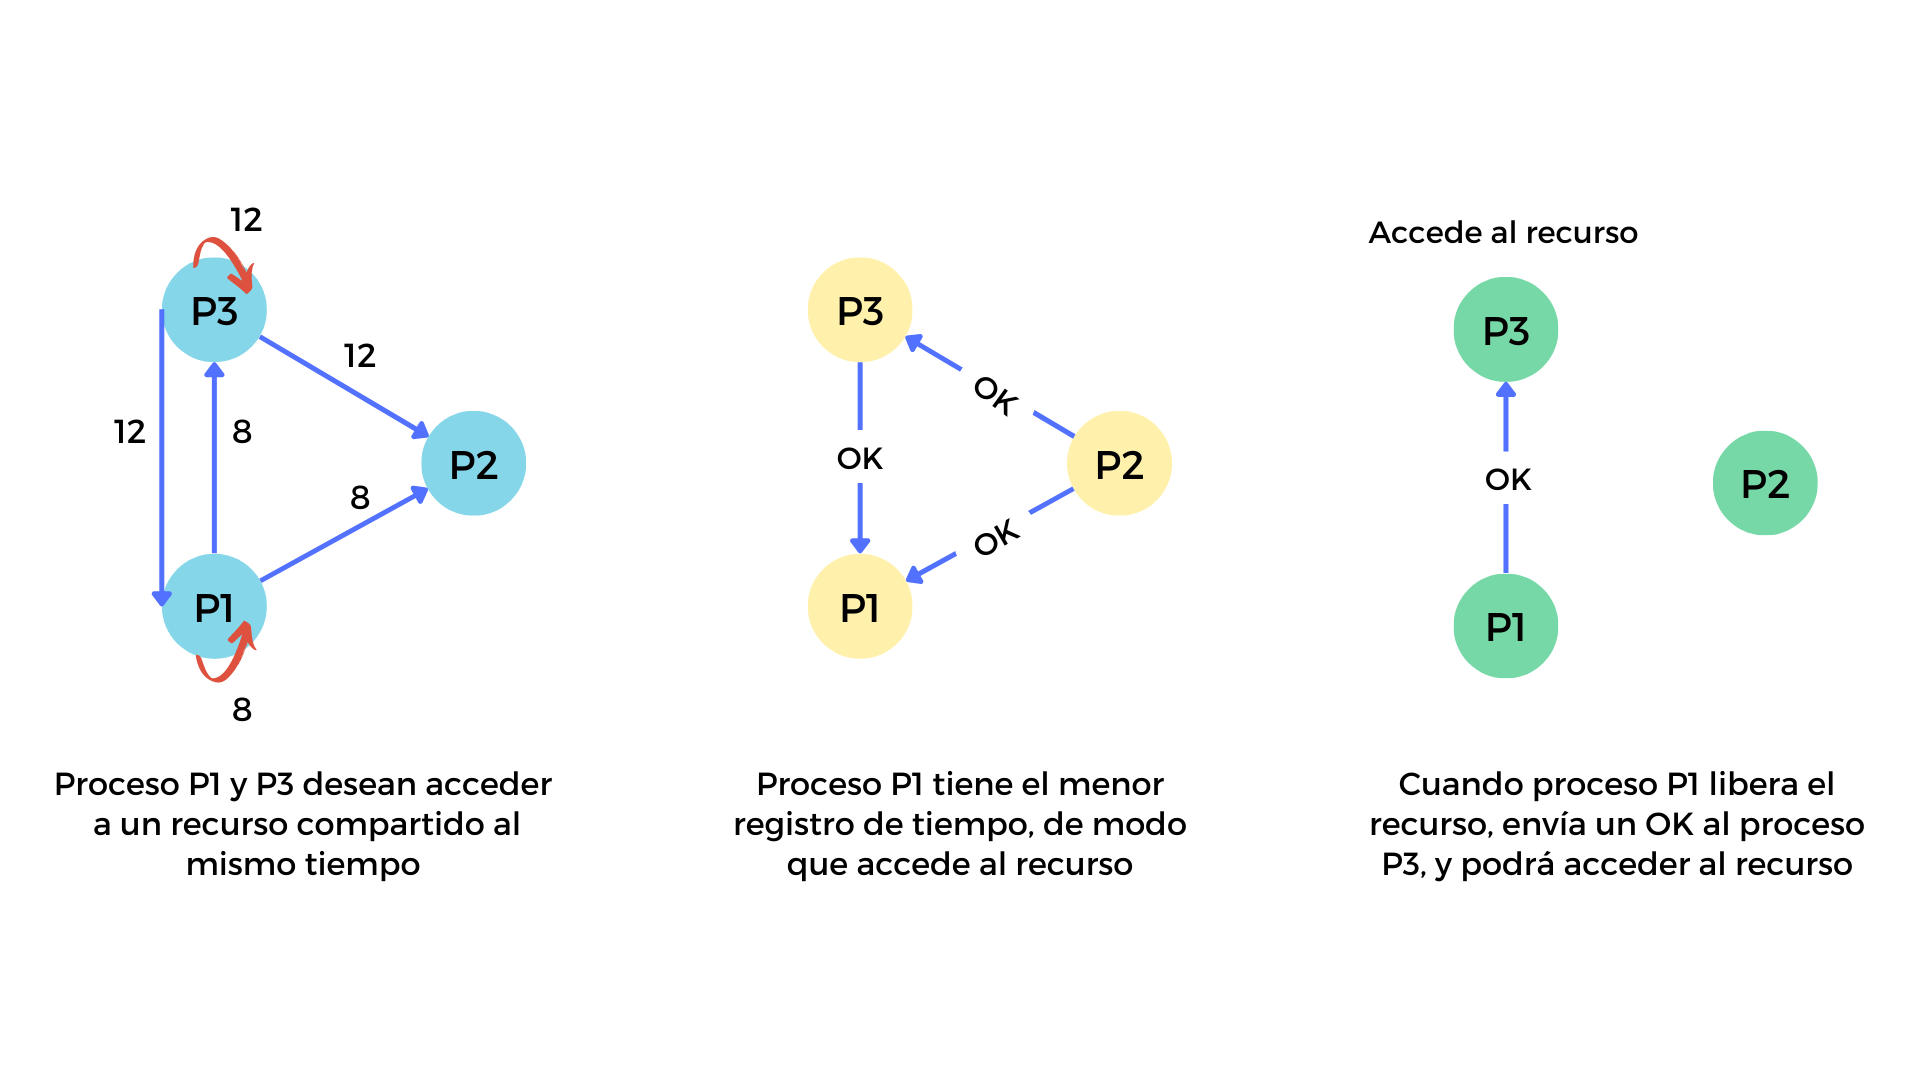
\includegraphics[width=0.8\linewidth] {8/C/10.png} 
 	\caption{ Algoritmo de Ricart-Agrawala.}
 	\label{fig:alg-Ricart-Agrawala}
 		\end{center}
 \end{figure}
 

%----------------------------------------------------------------------
 
	El algoritmo Ricart-Agrawala requiere la invocación de $2 (N - 1)$ mensajes por ejecución de sección crítica.  
 
 Su desventaja es su  enfoque no confiable: la falla de cualquiera
de los nodos del sistema puede detener el progreso del sistema. En esta situación, el proceso morirá de hambre.

Este  problema de falla del nodo se puede 	resolver detectando la falla después de un 	tiempo de espera.

El Rendimiento:
	\begin{enumerate}
		\item El retardo de sincronización es igual al
		tiempo máximo de transmisión de mensajes
		
		\item 	Requiere $2 (N - 1)$ mensajes por ejecución
		de sección crítica.
	\end{enumerate}
	
	%---------------------------------------------------------------
	\subsubsection{Algoritmo de Suzuki-Kazami}
	%---------------------------------------------------------------
	\index{ Algoritmo de Suzuki-Kazami}
	
	El algoritmo de Suzuki-Kazami \cite{Suzuki1985} es una modificación del algoritmo Ricart-Agrawala, un algoritmo basado en permisos   que utiliza mensajes de SOLICITUD y RESPUESTA para garantizar la exclusión mutua.
	
	En este algoritmo se presenta un método en el que se modifica la antigüedad y también se entrega la sección crítica a otro nodo enviando un solo mensaje de PRIVILEGIO. Entonces, el nodo que tiene el PRIVILEGIO puede usar la sección crítica. Si un proceso quiere ingresar a su sección crítica y no tiene el token, transmite un mensaje de solicitud a todos los demás procesos del sistema. El proceso que tiene el token, si no se encuentra actualmente en una sección crítica, enviará el token al proceso solicitante. 	Cada solicitud de sección crítica contiene un número de secuencia. Este número de secuencia se utiliza para distinguir las solicitudes antiguas de las actuales.
	%%%%
	
	\paragraph{Estructura de Datos y notaciones}
	\begin{itemize}
		\item 	Una matriz de enteros $RN[1…N]$
		Un sitio $S_{i}$ mantiene $RN_{i}[1…N]$, donde $RN_{i}[j]$ es el mayor número de secuencia recibido hasta el momento a través del mensaje SOLICITUD del sitio $S_{i}$.
		\item Una matriz de enteros $LN[1…N]$
		El token guarda en esta matriz. $LN[J]$ el número de secuencia de la solicitud que el sitio $S_{j}$ ejecutó recientemente.
		\item Una cola $q$
		El token utiliza esta estructura de datos para mantener un registro de la identificación de los sitios que esperan el token.
	\end{itemize}
	
	\paragraph{Ingreso a la secci\'on cr\'itica}
	
	\begin{itemize}
		\item  	Cuando un sitio $S_{i}$ desea ingresar a la sección 	crítica y no tiene el token, incrementa su número de secuencia $RN_{i}[i]$ y envía un mensaje de solicitud $SOLICITUD_{(i, sn)}$ a todos los demás sitios para solicitar el token.
 		$sn$ es el valor de actualización de $RN_{i}[i]$
		\item Cuando un sitio $S_{j}$ recibe el mensaje de solicitud  $SOLICITUD_{(i, sn)}$ del sitio $S_{i}$, establece $RN_{j}[i]$ al máximo de $RN_{j}[i]$ y sn, es decir, $RN_{j}[i] = max(RN_{j}[i], sn)$.
		\item Después de actualizar $RN_{j}[i]$, el sitio $S_{j}$ envía el token al sitio $S_{i}$ si tiene token y $RN_{j}[i] = LN[i] + 1$
	\end{itemize}
	
	\paragraph{Ejecutar la sección crítica}
		
	El nodo $S_{i}$ ejecuta la sección crítica si ha adquirido el token.
	
\paragraph{	Liberar la sección crítica}
	Después de terminar la ejecución, el nodo $S_{i}$ sale de la sección crítica y hace lo siguiente:
	
	\begin{itemize}
		\item Establece $LN[i] = RN_{i}[i]$ para indicar que su solicitud de sección crítica $RN_{i}[i]$ ha sido ejecutada
		\item Para cada nodo $S_{i}$, cuyo $ID$ no está presente en la cola de tokens $Q$, agrega su $ID$ a $Q$ si $RN_{i[}j] = LN[j] + 1$ para indicar que el sitio $S_{j}$ tiene una solicitud pendiente.
		\item Después de la actualización anterior, si la cola $Q$ no está vacía, extrae una $ID$ de sitio de la $Q$ y envía el token al sitio indicado por la $ID$ extraída.
		\item Si la cola $Q$ está vacía, conserva el token
\end{itemize}

 \paragraph{Rendimiento}
 
 
 
El algoritmo requiere  la invocación de $0$ mensajes si el sitio ya tiene el token inactivo en el momento de la solicitud de la sección crítica o un máximo de $N$ mensajes por ejecución de la sección crítica. Este $N$ mensajes implica:
\begin{itemize}
	\item (N – 1) mensajes de solicitud
	\item 1 mensaje de respuesta
\end{itemize}


%----------------------------------------------------------------------
\subsection{Algoritmos basados en Elecciones}
%----------------------------------------------------------------------
\index{ algoritmo basado en elecciones}
%----------------------------------------------------------------------
El objetivo de los algoritmos basados en elecciones es el de elegir un proceso único para que tome un determinado rol o para decidir una determinada acción $n $

Entre sus aplicaciones estan las de:
	\begin{itemize}
		\item Elegir un nuevo servidor si se cae el actual 
		\item Elegir un nuevo proceso para entrar en una sección crítica 
		\item Elegir el proceso menos activo (balanceo de carga) 
		\item Elegir el proceso con la copia más reciente (réplicas)
	\end{itemize}	
 

%----------------------------------------------------------------------
Los algoritmos basados en Elecciones operan as\'i:	
	\begin{itemize}
		\item Un proceso convoca elecciones cuando lleva a cabo una acción que inicia el algoritmo de elección 
		\item Puede haber $N$ elecciones concurrentes 
		\item Un proceso siempre tiene uno de estos dos roles: 
		\begin{enumerate}
			\item Participante: comprometido en una ejecución del algoritmo 
			\item No participante: no comprometido en ninguna ejecución
		\end{enumerate}			 
		\item El proceso elegido debe ser único, incluso en elecciones concurrentes)
	 
		\item   Todos los procesos tienen un identificador 
		Único para el conjunto 
		\item El proceso elegido es aquél de mayor identificador 
		Variable elegido 
		\item Cada proceso $p_{i}$ mantiene una variable que contiene el identificador del proceso elegido 
		\item Cuando el proceso se convierta en participante, fija la variable al valor especial $\pm$, indicando que no hay consenso todavía
		
	\end{itemize}	
 
%----------------------------------------------------------------------

\subsubsection{Algoritmos de Anillo basado en Elecciones}
\index{ algoritmo de anillo basado en elecciones}
%----------------------------------------------------------------------
 En el algoritmo de Anillo basado en Elecciones \cite{Chang1979} se sigue el siguiente proceso:
 
	\begin{enumerate}
		\item Inicialmente todos los procesos son \textit{\textbf{no participantes}}.
		\item Cualquier proceso $P$ decide arrancar una elección en cualquier momento.
		\item. Proceso $P$ se pone en estado \textbf{participante} y envía un mensaje de elección $M$ a su vecino.
		\item El mensaje $ M$ contiene el \textbf{ID} del proceso que ha iniciado la elección.
		\item Cuando el vecino recibe el mensaje de elección $M$, establece su estado como participante y comprueba el \textbf{ID} del mensaje.
		\item Si es mayor que su propio \textbf{ID}, entonces se lo envía directamente a su vecino.
		\item Si su \textbf{ID} es mayor al \textbf{ID} recibido, entonces lo coloca en el mensaje $M$ y lo envía a su vecino.				
 
		\item Así se circula el mensaje $M$ sucesivamente hasta que llega a un proceso $P_{n}$ que comprueba que el \textbf{ID} recibido es el propio. Eso indica que ha sobrevivido el mayor \textbf{ID}, que es la del proceso  $P_{n}$ .
		\item Entonces, este proceso  $P_{n}$  es el coordinador y lo notifica a su vecino Cuando un proceso recibe un mensaje de coordinador debe de poner su estado como \textbf{no participante }y enviar el mensaje a su vecino.
		\item Cuando el mensaje de coordinador retorna al proceso que lo emitió (coordinador), entonces todos los procesos saben quién es el coordinador y todos quedan en estado \textbf{no participantes}.
	\end{enumerate}		
	
	En la Figura \ref{fig:alg-Anillo-eleccion} se muestra paso a paso como opera el algoritmo.	 
 
Los algoritmos de Anillo basado en Elecciones se usan cuando:
 
	\begin{enumerate}		
		
		\item  Los procesos están física o lógicamente ordenados en anillo.
		\item No se conoce el número total de procesos (n).
		\item Cada proceso se comunica con su vecino (izquierda o derecha).
	\end{enumerate}			 
 
 \paragraph{Extinci\'on del Proceso}	
	\begin{enumerate}
		\item En caso de que dos procesos inicien al mismo tiempo una elección y se envíen mensajes de elección, un proceso en estado de \textbf{participante} debe de verificar el \textbf{ID} del proceso que envía el mensaje de elección.
		\item  Si es menor al propio, el mensaje se descarta. Así, todos 	los mensajes de elección se extinguirán, excepto el que lleva el \textbf{ID} más alto.
	\end{enumerate}	
 
%----------------------------------------------------------------------
 
\begin{figure}[h]%
		\begin{center}
	\includegraphics[width=0.8\linewidth] {8/C/3.png} 
	\includegraphics [width=0.8\linewidth]{8/C/4.png} 
	\caption{Algoritmo de Anillo basado en Elecci\'on.}
	\label{fig:alg-Anillo-eleccion}
		\end{center}
\end{figure}

%----------------------------------------------------------------------
\subsubsection{Algoritmos de \textit{Bully}}
\index{ algoritmo de bully}
%---------------------------------------------------------------------
 Las premisas del algoritmos de \textit{Bully} \cite{GarciaMolina1982}

	\begin{enumerate}				
		\item  El sistema es síncrono y utiliza tiempo de espera para la identificación de fallas en los procesos.
		\item Se permite que los procesos se bloqueen durante la ejecución del algoritmo.
		\item La entrega de mensajes entre procesos se supone fiable y dentro de un periodo máximo.
		\item Los procesos están ordenados, tienen un único identificador (\textbf{IDs}) conocido y se sabe cuántos procesos existen.
	\end{enumerate}			 

Los tipos de mensajes entre los procesos:
	\begin{enumerate}
		\item Mensaje de Elección:seleccionar un nuevo coordinador.
		\item Mensaje de Respuesta: respuesta al mensaje de elección.
		\item Mensaje de Coordinador: comunica el ID del proceso seleccionado como coordinador.
	\end{enumerate}	
 
%----------------------------------------------------------------------
El algoritmos de \textit{Bully} opera de la siguiente manera:
 
	\begin{enumerate}				
		\item  Un proceso $x$ manda un mensaje de elección a todos aquellos procesos que tengan un identificador más grande cuando detecta que el coordinador ha fallado.
		\item El proceso $x$ espera los votos y, si ningún voto (ok) llega después de un cierto tiempo, el proceso $sx$ se declara coordinador, y envía el mensaje de coordinador a los procesos con identificador más pequeño que el suyo.
		\item Si un voto llega (aunque pueden llegar varios votos), puede ser que otro coordinador sea declarado ganador.
		\item  Si un proceso recibe un mensaje de elección, envía un voto y otra elección empieza.
		\item Cuando un coordinador que ha fallado regresa, empieza una elección y puede volver a readquirir el control, aunque exista un coordinador actual.
	\end{enumerate}			 
 
%---------------------------------------------------------------------
  En la Figura \ref{fig:alg-Bully} se ilustra el proceso de elecci\'on del coordinador que propone el algoritmo del Bully.
 
\begin{figure}[h]%
	\begin{center}
	
	\includegraphics [width=0.8\linewidth] {8/C/7.png} 
	\includegraphics [width=0.8\linewidth]{8/C/8.png}
	\includegraphics [width=0.8\linewidth]{8/C/9.png}  
		\caption{Algoritmo de Bully}
		\label{fig:alg-Bully}
		\end{center}
		\end{figure}
 

%----------------------------------------------------------------------
 
%-----------------------------------------------------------------
\subsubsection{Algoritmo Generales Bizantinos}
\index{ algoritmo de generales bizantinos}
%----------------------------------------------------------------- 
El problema de los generales bizantinos  \cite{Lamport1982}  plantea que un grupo de generales sitia una ciudad y deben ponerse de acuerdo a través de un plan de ataque para atacar o retirarse.
Los generales solo se comunican a través de mensajes a los otros generales.   Uno de ellos, el comandante, da las órdenes.  	Los otros, tenientes, deben de decidir si atacar o retirarse. 
Sin embargo, uno o más de los generales puede ser un traidor o pueden fallar. 
	 
	Esta traición puede verse de dos formas:
	\begin{enumerate}				
		\item  
		Los mensajes pueden no llegar o, dicho de otra manera, las comunicaciones no son confiables.
		\item Un general traidor puede mentir, es decir, un nodo puede fallar de manera impredecible
	\end{enumerate}			 

%------------------------------------------------------------------

\paragraph{Algoritmo Generales Bizantinos.  Caso 1: tres generales}
	\textbf{Escenario}:  un comandante y dos tenientes, y uno 	de ellos es traidor. ¿Pueden llegar a un consenso?, es decir, ¿acordar \textbf{atacar} o \textbf{retirarse}?
	Se asume que el  comandante es el traidor  
	\begin{enumerate}				
		\item	
		El  comandante indicará al teniente 1 \textbf{atacar} y al teniente 2 \textbf{retirarse}. 
		Tenientes verifican la orden recibida comunicándose entre ellos.
		\item Teniente 1 al teniente 2 que recibió  \textbf{atacar}
		\item Teniente 2 al teniente 1 que recibió  \textbf{retirarse}. 
		\item Tenientes  deducen que el comandante  es traidor y no  pueden tomar una decisión consuensada.
	\end{enumerate}			 
 
 Ver la Figura \ref{fig:alg-bizantino-1} con la illustraci\'on de la operaci\'on del algoritmo.
%-------------------------------------------------------------------
 

 \begin{figure}[h]%
 		\begin{center}
	\includegraphics[width=0.8\linewidth] {8/C/5.png} 
		\caption{Algoritmo de Generales Bizantinos. Caso 1.}
		\label{fig:alg-bizantino-1}
			\end{center}
	\end{figure}

%-------------------------------------------------------------------
\paragraph{ Algoritmos Generales Bizantino. Caso 2- Cuatro Generales}

Se presentan dos escenarios:
 
	\textbf{Escenario 1}:  un comandante y dos tenientes, y uno de ellos es traidor. ¿Pueden los generales leales llegar a un consenso?, es decir, ¿acordar \textbf{atacar} o \textbf{retirarse}?
	\begin{enumerate}				
		\item 	Asume que el\textbf{comandante} es el traidor  			
		\item Independiente de las órdenes que reciban los tenientes  del  comandante, ellos intercambian informaci\'on entre sí, de tal manera que los tres recibirán tres mensajes.
		\item Al decidir por la mayoría de las órdenes recibidas, los tres tenientes tomarán la misma decisión. En este caso, \textbf{atacar}
	\end{enumerate}			 
 
%------------------------------------------------
%------------------------------------------------
 
	\textbf{Escenario 2}:  un general y dos tenientes, y uno de ellos es traidor. ¿Pueden los generales leales llegar a un consenso?, es decir, ¿acordar \textbf{atacar} o \textbf{retirarse}?
	\begin{enumerate}				
		\item Asume que el\textbf{ teniente 3} es el traidor  			
		\item El comandante envía a todos los tenientes la orden de \textbf{atacar}. 
		\item Esta orden es retransmitida por los tenientes 1 y 2 a los demás
		\item Teniente 3 cambia la orden recibida y envía a los tenientes generales 1 y 2 la orden de \textbf{retirarse}. 
		\item Esto no cambia la decisión consensuada de los tenientes 1 y 2: por mayoría deciden atacar.
	\end{enumerate}			 
 
%------------------------------------------------
 	
	\begin{figure}[h]%
			\begin{center}
		\includegraphics [width=0.8\linewidth]{8/C/6.png} 
		\caption{Algoritmo de Generales Bizantinos. Caso 2.}
		\label{fig:alg-bizantino-2}
			\end{center}
	\end{figure}
	
En  la Figura \ref{fig:alg-bizantino-2}  se muestra el intercambio de mensaje entre los generales para el caso de cuatro generales. 	
	

%%	\cite{Vitillo2021} 	\cite{Raptis2020} 	\cite{Shetty2019} 	  \cite{Limoncelli2014}  \cite{Verissimo2012} 	\cite{Czaja2018} \cite{Coulouris2011}

\section{Caso de Estudio. Elecci\'on del Lider}

\index{caso de estudio!elecci\'on del lider} \index{algoritmo de elección de líder de Raft}
Un problema muy común es la elección de líder, donde los nodos que forman parte de un sistema distribuido necesitan elegir un nodo entre ellos para que actúe como su líder, coordinando el funcionamiento de todo el sistema. Un ejemplo de esto es el esquema de replicación de un solo maestro que se presentó anteriormente en el libro. Este esquema se basa en que un nodo, designado como primario, será el responsable de realizar operaciones de actualización de datos y los otros nodos, designados como secundarios, realizarán el seguimiento con las mismas operaciones. Sin embargo, para poder hacerlo, el sistema primero necesita seleccionar el nodo primario, lo cual es un proceso llamado elección de líder. Dado que todos los nodos prácticamente están de acuerdo en un único valor, la identidad del líder, este problema puede modelarse fácilmente como un problema de consenso  \cite{Vitillo2021}


El algoritmo de elección de líder de Raft \cite{Raptis2020} se implementa con una máquina de estados en la que un proceso se encuentra en uno de tres estados (ver Figura \ref{fig:alg-lider}):

\begin{itemize}
	\item el estado seguidor, en el que el proceso reconoce a otro como líder;
	\item el Estado candidato, en el que se inicia el proceso de una nueva elección proponiéndose como líder;
	\item o el estado líder, en el que el proceso es el líder.
\end{itemize}

En Raft, el tiempo se divide en períodos electorales de duración arbitraria. Un período electoral se representa con un reloj lógico, un contador numérico que sólo puede aumentar con el tiempo. Un mandato comienza con una nueva elección, durante la cual uno o más candidatos intentan convertirse en líder. El algoritmo garantiza que para cualquier término haya como máximo un líder. Pero, en primer lugar, ¿qué desencadena una elección?


\begin{figure}[h]%
		\begin{center}
	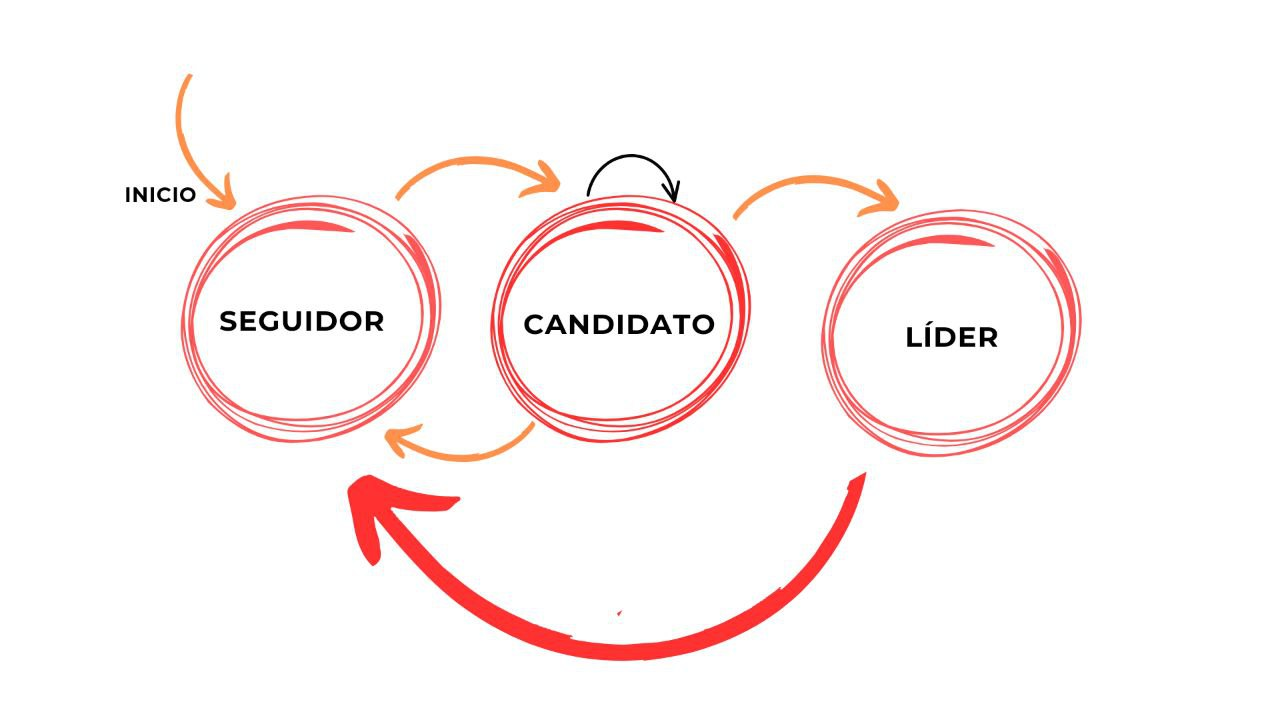
\includegraphics[width=0.8\linewidth] {8/Raft.jpg} 
	\caption{Algoritmo de elecci\'on del lider Raft.}
	\label{fig:alg-lider}
		\end{center}
\end{figure}

Cuando el sistema se inicia, todos los procesos comienzan su recorrido como seguidores. Un seguidor espera recibir un mensaje periódico del líder que contiene el período electoral en el que fue elegido el líder. Si el seguidor no recibe ningún mensaje dentro de un período de tiempo determinado, se activa un tiempo de espera y se presume que el líder está muerto. En ese punto, el seguidor comienza una nueva elección incrementando el período electoral actual y haciendo la transición al estado candidato. Luego vota por sí mismo y envía una solicitud a todos los procesos del sistema para que voten por él, sellando la solicitud con el período electoral actual.

El proceso permanece en el estado candidato hasta que sucede una de tres cosas: gana las elecciones, otro proceso gana las elecciones o pasa un tiempo sin ganador.

\begin{itemize}
	\item El candidato gana las elecciones: el candidato gana las elecciones si la mayoría de los procesos del sistema votan a favor. Cada proceso puede votar por como máximo un candidato en un mandato por orden de llegada. Esta regla de la mayoría impone que como máximo un candidato pueda ganar un mandato. Si el candidato gana las elecciones, pasa al estado líder y comienza a enviar mensajes a los demás procesos.
	\item Otro proceso gana las elecciones: si el candidato recibe un mensaje de un proceso que afirma ser el líder con un mandato mayor o igual al mandato del candidato, acepta al nuevo líder y regresa al estado seguidor. Si no, continúa en el estado candidato. Quizás se pregunte cómo pudo suceder eso; por ejemplo, si el proceso de candidatura se detuviera por cualquier motivo, como por una pausa prolongada de la Asamblea General, para cuando se reanude, otro proceso podría haber ganado las elecciones.
	\item Pasa un período de tiempo sin un ganador: es poco probable, pero posible, que varios seguidores se conviertan en candidatos simultáneamente y ninguno logre recibir la mayoría de los votos; esto se conoce como votación dividida. Cuando eso suceda, el candidato eventualmente expirará y comenzará una nueva elección. El tiempo de espera de las elecciones se elige aleatoriamente entre un intervalo fijo para reducir la probabilidad de otra votación dividida en las próximas elecciones.

\end{itemize}

 


%\paragraph{Bloqueo distribuido}

%La mayoría de los sistemas distribuidos reciben múltiples solicitudes simultáneas y necesitan realizar algún control de concurrencia para evitar inconsistencias de datos debido a la interferencia entre estas solicitudes. Uno de estos métodos de control de concurrencia es el bloqueo, pero su uso en el contexto de un sistema distribuido conlleva muchos casos extremos, lo que añade mucho riesgo. Por supuesto, el bloqueo distribuido también se puede modelar como un problema de consenso, donde los nodos del sistema acuerdan un valor único, que es el nodo que mantiene el bloqueo.

%\paragraph{Transmisión atómica}

%Otro problema comúnmente citado es la transmisión atómica, que se ocupa de permitir que un conjunto de nodos transmitan mensajes simultáneamente y al mismo tiempo garantizar que todos los destinos los entreguen consistentemente en exactamente la misma secuencia a pesar de la posible presencia de nodos defectuosos. Este problema también equivale al consenso, como también se demostró en investigaciones anteriores [6][36]. La razón por la que describimos estos problemas y demostramos cómo se pueden modelar como un problema de consenso es para que usted pueda apreciar el valor de esta abstracción y comprender que resolver el problema de consenso puede proporcionar soluciones a muchos más problemas.

